% ****** Start of file apssamp.tex ******
%
%   This file is part of the APS files in the REVTeX 4.1 distribution.
%   Version 4.1r of REVTeX, August 2010
%
%   Copyright (c) 2009, 2010 The American Physical Society.
%
%   See the REVTeX 4 README file for restrictions and more information.
%
% TeX'ing this file requires that you have AMS-LaTeX 2.0 installed
% as well as the rest of the prerequisites for REVTeX 4.1
%
% See the REVTeX 4 README file
% It also requires running BibTeX. The commands are as follows:
%
%  1)  latex apssamp.tex
%  2)  bibtex apssamp
%  3)  latex apssamp.tex
%  4)  latex apssamp.tex
%
\documentclass[%
%reprint,                                   %%%%%%%%%%% this one makes it look like a paper
%superscriptaddress,
%groupedaddress,
%unsortedaddress,
%runinaddress,
%frontmatterverbose, 
preprint,                                  %%%%%%%%%%%%%%%% this one for drafting
%showpacs,preprintnumbers,
nofootinbib,
%nobibnotes,
%bibnotes,
 amsmath,amssymb,
 aps,
%pra,
%prb,
%rmp,
%prstab,
%prstper,
%floatfix,
]{revtex4-1}


%%%%%%%%%%%%%%%%%%%%%%%
\usepackage{lineno}
\linenumbers % add line numbers, draft
%%%%%%%%%%%%%%%%%%%%%%%


%%%%%%%%%%%%%%%%%%%%%%%%%%%%%%%%%%%%%%%%%%%%%%%
\usepackage{graphicx}% Include figure files                  \usepackage[draft]{graphicx}
%%%%%%%%%%%%%%%%%%%%%%%%%%%%%%%%%%%%%%%%%%%%%%%


%%%%%%%%%%%%%%%%%%%%%%%%%%%%%%%
\usepackage[printfigures]{figcaps} % send figures to end
%%%%%%%%%%%%%%%%%%%%%%%%%%%%%%%

%%%%%%%%%%%%%%%%%%%%%%%%%%%%%%%%%%%%%%%%%%%%%%%
\usepackage{natbib} % allows author names in text, delete when finished?
%%%%%%%%%%%%%%%%%%%%%%%%%%%%%%%%%%%%%%%%%%%%%%%


\usepackage{dcolumn}% Align table columns on decimal point
\usepackage{bm}% bold math
%\usepackage{hyperref}% add hypertext capabilities
%\usepackage[mathlines]{lineno}% Enable numbering of text and display math
%\linenumbers\relax % Commence numbering lines

%\usepackage[showframe,%Uncomment any one of the following lines to test 
%%scale=0.7, marginratio={1:1, 2:3}, ignoreall,% default settings
%%text={7in,10in},centering,
%%margin=1.5in,
%%total={6.5in,8.75in}, top=1.2in, left=0.9in, includefoot,
%height=10in,a5paper,hmargin={3cm,0.8in},
%]{geometry}

\begin{document}

\newcommand{\wmk}{Wm$^{-1}$K$^{-1}$}

%\preprint{APS/123-QED}

\title{Finite size effects in simulations of thermal conductivity under lower mantle conditions}% Force line breaks with \\

\author{Ben Todd}
 \email{Corresponding  author: ee10bt@leeds.ac.uk}
\author{Stephen Stackhouse}
\author{Andrew M. Walker}
\author{Jon E. Mound}

\affiliation{School of Earth and Environment, University of Leeds, United Kingdom}

\date{\today}% It is always \today, today,
             %  but any date may be explicitly specified

\begin{abstract}

%2Knowledge of thermal conductivity is important for modelling the deep earth, but can not be measured experimentally at core mantle boundary conditions. Atomic scale simulations sidestep experimental limitations, but system size must be chosen carefully in order to determine accurate conductivity values.

3? Here we investigate the effects of finite simulation size and show how conductivity can be estimated incorrectly when using the direct method. EXTRAPOLATION PROCEDURE

2?WE FIND OTHER STUDIES MAY HAVE DONE STUFF WRONG BY NOT CONSIDERING FSE

%2 Classical molecular dynamics approaches are utilised, with the intention of constraining appropriate system parameters. %for future (first principles) studies.

ADD RESULTS

TO DO:

SCALING LAW

\end{abstract}

\maketitle


%%%%%%%%%%%%%%%%%%%%%%%%%%%%%%%%%%
%\onecolumngrid % make one column, delete to go back to two IGNORE THIS, USE document class
%%%%%%%%%%%%%%%%%%%%%%%%%%%%%%%%%%


\section{\label{sec:intro}Introduction}

\subsection{\label{sec:intro.intro}Intro Intro (remove this subsection header later)}

%\textsc{\char13}

%1? Knowledge of the thermal conductivity of solids is key in a wide range of technological applications and for our understanding of natural systems. For example, in the Earth's lower mantle thermal conductivity controls the nature of planetary convection (\citet{Tosi2013}), and the heat flux out of the core which powers the geotherm. Low thermal conductivities are required in thermoelectric materials, to maximise the efficiency of heat-electricity conversion (\citet{Snyder2008}).

%2 A range of atomic scale simulation methods are available to determine the lattice thermal conductivity of materials. These are invaluable for calculating thermal conductivity at conditions of which experiments are difficult, e.g. the extreme conditions found in the Earth's lower mantle (pressures and temperatures up to 136~GPa and 4000~K at the core-mantle boundary). 


%1 (MOVE - to where though?) Many studies assume lowermost mantle thermal conductivity to be 10~\wmk~(e.g. \citet{Lay2008}), but uncertainty in the extrapolation of results made at low pressures and temperatures gives a range of 4~-~16 \wmk~(\citet{Brown1986, Osako1991, Hofmeister1999, Goncharov2009, Manthilake2011, Ohta2012}).

%MENTION THEORETICAL CALCULATIONS HERE? TRYING TO MAKE UNCERTAINTY IN EXPERIMENTS OBVIOUS, GOING TO TALK ABOUT THEORETICAL RESULTS JUST FOR PURE BRIDG 
 
%\textemdash

%1 %Thermal conductivity determines whether a material is a conductor or insulator of heat, both of which have many technological applications (such as in solar panels REF[that guy from Huddersfield/N8?]).

%1 %Thermal conductivity in the deep Earth influences dynamic processes such as mantle convection and heat loss from the core (\citet{Lay2008}). The value of thermal conductivity in the deep mantle is uncertain, because of the need to extrapolate experimental results (e.g. \citet{Hofmeister1999} OHTA MANTHILAKE?). 

%1 %For many studies lowermost mantle thermal conductivity has been assumed to be 10~\wmk (\citet{Lay2008}). More recent experiments (and theoretical calculations) have produced estimates of thermal conductivity close to the core mantle boundary (CMB) of 4~\textemdash~16 \wmk (\citet{Goncharov2009,Lay2008,Hofmeister1999,Brown1986}). ADD REFERENCES FOR THEORETICAL CALCULATIONS

%1 %The lower mantle encompasses the region between the mantle transition zone (660~km deep, $\sim$1900~K, $\sim$25~GPa) and the CMB(2891~km deep, $\sim$4000~K, $\sim$136~GPa). The composition of this region can be approximated as 80\% MgSiO$_3$/magnesium silicate perovskite (bridgmanite) and 20\% MgO/magnesium oxide (periclase)[not sure how to write mineral formulae/names], both of which are insulators and past their Debye temperatures at lower mantle conditions.

\subsection{\label{sec:intro.pre}Pre-intro to methods (remove this subsection header later)}

%2 \citet{Stackhouse2010} review different methods to compute thermal conductivity, in the present work we focus on two of these:(1) Equilibrium molecular dynamics based on the Green-Kubo relations to determine the thermal conductivity from heat flux fluctuations and their time-dependence (\citet{Green1954,Kubo1957,Kubo1966,Schelling2002}REMOVE SCHELLING REFERENCE?). (2) The non-equilbrium molecular dynamics-based ``direct method'', where thermal conductivity is calculated from an imposed heat flux and corresponding temperature gradient via Fourier's Law (\citet{Muller-Plathe1997,Nieto-Draghi2013}).

%2 %The important common atomic scale methods are: 
%(3) Anharmonic lattice dynamics. [\citet{Tang2009}] %(BTE)CHERNATYNSKIY and PHILLPOT 2010?
%(4) Combined quasiharmonic lattice dynamics and molecular dynamics method [\citet{DeKoker2009}].

\subsection{\label{sec:intro.question}The question/motivation (remove this subsection header later)}

%2 Considering systems of varying size, length-dependent conductivities are obtained from the direct method and extrapolated to the bulk material (\citet{Schelling2002}). The validity of this extrapolation procedure have been called into question (e.g. \citet{Sellan2010}), when a linear trend cannot be fit through the length-dependent conductivities [THIS WHOLE PARAGRAPH IS WISHY-WASHY, SPECIFIC THINGS TO AS-YET-UNDISCUSSED DIRECT METHOD, NOT GENERAL STATEMENTS]. We describe finite-size effects (FSE) which cause the conductivity result of a simulation to diverge from the value expected by a linear trend, and offer a comparison with results obtained from the Green-Kubo method. The two methods have previously been compared (e.g. \citet{Schelling2002} [[[REFERENCED EARLIER IN THIS PARAGRAPH, THIS OKAY?]]] ), and have been found to give results in good agreement. [[[IMPORTANT FOR ABSTRACT]]]




\subsection{\label{sec:intro.brdg}Bridgmanite (remove this subsection header later)}

%(WHY ELSE IS BRIDG INTERESTING, OUTSIDE OF EARTH APPLICATIONS)(BRIDG ELECTRICAL/RADIATIVE CONDUCTIVITY)(HOW DOES BRIDG COMPARE TO MATERIALS IN OTHER FSE STUDIES)
%2 Bridgmanite, or MgSiO$_3$ (magnesium silicate) perovskite, comprises around 80\% (75\%? REF?) of the lower mantle (need to mention the other 20\%?), and is an insulator past its Debye temperature at all conditions relevant to the deep earth (TRUE? REF?). 

(((MOVE TO DISCUSSION?)))
%1 There have been several computational studies to calculate the lattice thermal conductivity of bridgmanite at CMB conditions. Our approach is similar to that of \citet{Ammann2014}, who use the direct method and interatomic potentials reporting a value of $\sim$8.5~\wmk. \citet{Stackhouse2015} again use the direct method but with density functional theory, yielding conductivity of 6.8~$\pm$~0.9~\wmk. Using Green-Kubo, \citet{Haigis2013} report a value of 12.4~$\pm$~2.0~\wmk for conditions of 3000~K, 139~GPa. \citet{Tang2014} and \citet{Dekura2013} employed first principles, anharmonic lattice dynamics techniques, obtaining values of $\sim$1~\wmk (CMB conditions) and 2.3~\wmk (for 4000~K and 100~GPa) respectively. These results are much lower than other studies, and could be because of LD TRUNCATION OF CONDUCTIVITY [CRITICAL ANALYSIS].








%1 %BEGIN COPY/PASTE FROM TRANSFER REPORT

%\citet{Osako1991} measured the lattice thermal conductivity of MgSiO$_3$ perovskite, using a modified \AA ngstrom method. They investigated a temperature range of 160 - 340~K at ambient pressure. At 300~K, a conductivity of 5.1~\wmk was obtained. This value is similar to that reported for chemical and structural analogues, MgSiO$_3$ enstatite (5.0~\wmk REF) and CaTiO$_{3}$ perovskite (4~\wmk REF). The authors extrapolated the value to mantle conditions, neglecting radiative thermal conductivity. They predicted a value of 3.0~\wmk just beneath the mantle transition zone at 1900~K, and 12.0~\wmk at the top of the D$^{\prime \prime}$ layer at 2500~K, a four-fold increase. 
%Thermal conductivity is highlighted as an important indictor of lowermost mantle structure, whether or not the D$^{\prime \prime}$ layer can behave as a thermal boundary between core and mantle. [not needed JM 150327]

%\par \citet{Manthilake2011} measured MgSiO$_3$ perovskite at 26~GPa and 473~-~1073~K, and periclase at 8 and 14~GPa between 373~-~1273~K. In order to estimate values of thermal conductivity at the top and bottom of D$^{\prime \prime}$ for a lower mantle compositional model of 4~perovskite~:~1~periclase, the authors extrapolated their measurements to high temperature and pressure. For an iron-free mantle, thermal conductivities of 18.9~$\pm$~1.6~\wmk and 15.4~$\pm$~1.4~\wmk are estimated for the top of D$^{\prime \prime}$ and CMB respectively. Similarly, for a mantle composition with Fe, thermal conductivities of 9.1~$\pm$~1.2~\wmk and 8.4~$\pm$~1.2~\wmk are calculated. This highlights the importance of impurities in controlling thermal conductivity in the lower mantle.

%\par \citet{Ohta2012} measured the lattice thermal diffusivity of MgSiO$_3$ perovskite and post-perovskite at room temperature and pressures up to 144~GPa (using a diamond-anvil cell (DAC) and light heating thermoreflectance). These results suggest a perovskite-dominant lowermost mantle would have conducitivity of around 11~\wmk, and that parts of the lowermost mantle where post-perovskite is stable will have a conductivity approximately 60\% higher. The authors suggest that these differences in conductivity between phases will not have a large effect on CMB heat flux, assuming the double-crossing perovskite phase model. %The lattice conductivity of \perovs perovskite is shown to increase with pressure and decrease with temperature as expected. The inclusion of impurities is expected to decrease lattice thermal conductivity.

%MANTHILAKE'S HIGH T RESULTS? CAN'T FIND REFERENCE?

%END COPY/PASTE FROM TRANSFER REPORT







\subsection{\label{sec:intro.end}Intro to rest of paper (remove this subsection header later)}

%1In section \ref{sec:theory} [[Section?]] we provide an overview of the methods and expand on issues.In section \ref{sec:methodology} we outline our computational approaches, for the non-equilibrium molecular dynamics direct method and equilibrium molecular dynamics Green-Kubo method. In section \ref{sec:results} we show convergence of computed conductivity with respect to simulation cell size and shape (AND PRESSURE/TEMPERATURE EFFECTS?). ALSO IN RESULTS, DISCUSS [P/T] SCALING LAW / THEORETICAL MODEL?In section \ref{sec:summary} we suggest parameters to be utilised in similar lower mantle studies, and discuss potential future work. 




\section{\label{sec:theory}Theory}

\subsection{\label{sec:theory.phon}Phonons (remove this subsection header later)}

PHYSICS JOURNAL LEVEL? 
 %1 Heat is transported as lattice virbrations, or phonons. The further phonons travel before scattering (mean free path, MFP) the more efficient the heat transport and thus higher the thermal condutivity. A number of effects (MENTION MATTHIESSEN'S RULE) cause phonons to scatter: (1) collisions with other phonons in the lattice, (2) boundaries or defects in the material, and (3) impurities in the atomic structure. 

% CHAPTER 2
The finite-size effects we describe are associated with (1), where simulation system sizes are too small to recreate the phonon-phonon scattering of the bulk material. The FSE observed for a material change with thermal conductivity/phonon MFP, and thus are pressure, temperature, and composition sensitive. Higher conductivity materials/conditions require larger systems to eliminate FSE (and vice versa) [[[BUT IS THIS TRUE? SHOULD IT BE IN THIS SECTION, OR DISCUSSION?]]]




\subsection{\label{sec:theory.direct}Direct method (remove this subsection header later)}

%%% ALL TO %2
The direct method is the computational implementation of a typical experiment to measure thermal conductivity, using Fourier\textsc{\char13}s law to relate heat flux (q) and temperature gradient ($\nabla{T}$) to thermal conductivity (k), 
\begin{equation}
q=-k \nabla{T} \label{fourier}.
\end{equation}

In the direct method energy is transferred from one group of atoms to another, creating hot and cold regions between which heat flows. The resultant temperature gradient is measured by calculating the temperature of individual groups of atoms along the direction of the heat flux. Simulation cells tend to be long relative to their cross-sectional area, defined as height by width. %(see Figure~\ref{fig:cell_dia}) 
Cell boundaries are periodic and the hot and cold sections are half the cell length apart, meaning heat flows in both directions from hot to cold (one of which is across the length-end periodic boundary). This results in two similar temperature gradients which can be averaged.

%\begin{figure}[h]
%  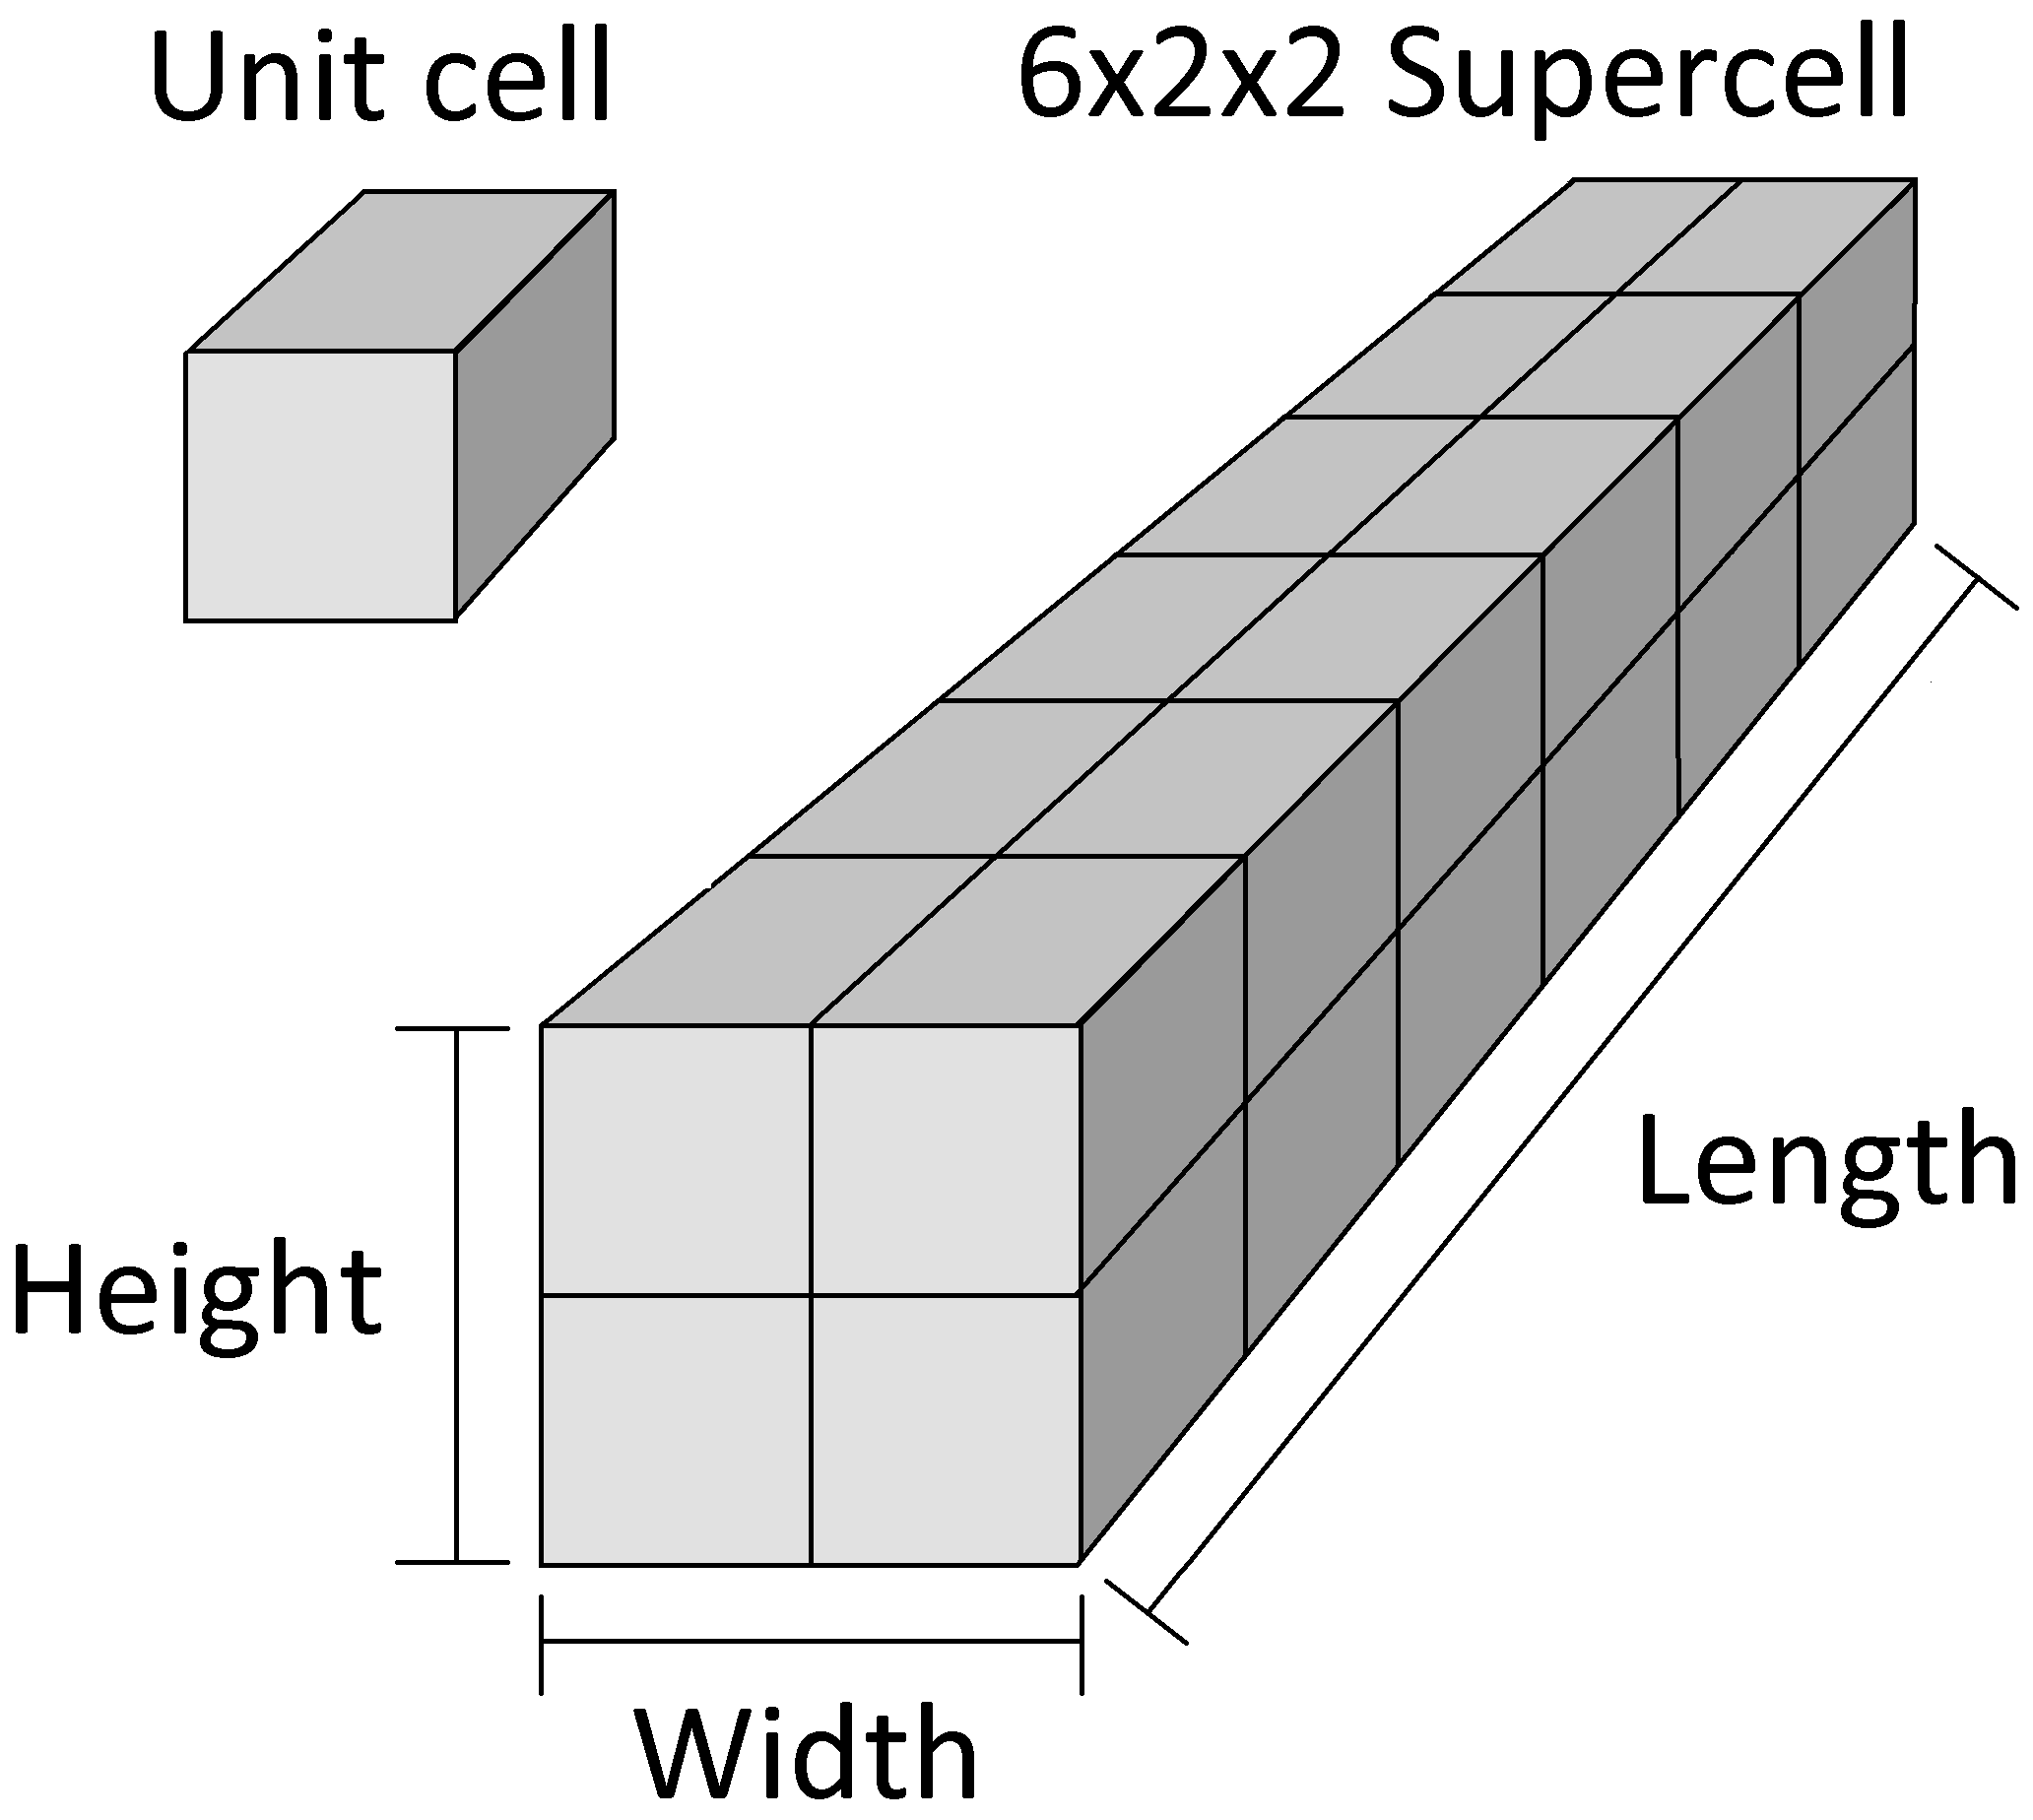
\includegraphics[width=\linewidth]{images/cell_diagram.png}
%  \caption{The unit cell represents the smallest box of atoms that can be replicated to produce a crystal structure. A supercell is an arrangement of unit cells.}
%\label{fig:cell_dia}
%\end{figure}

%%\begin{figure}[h]
%  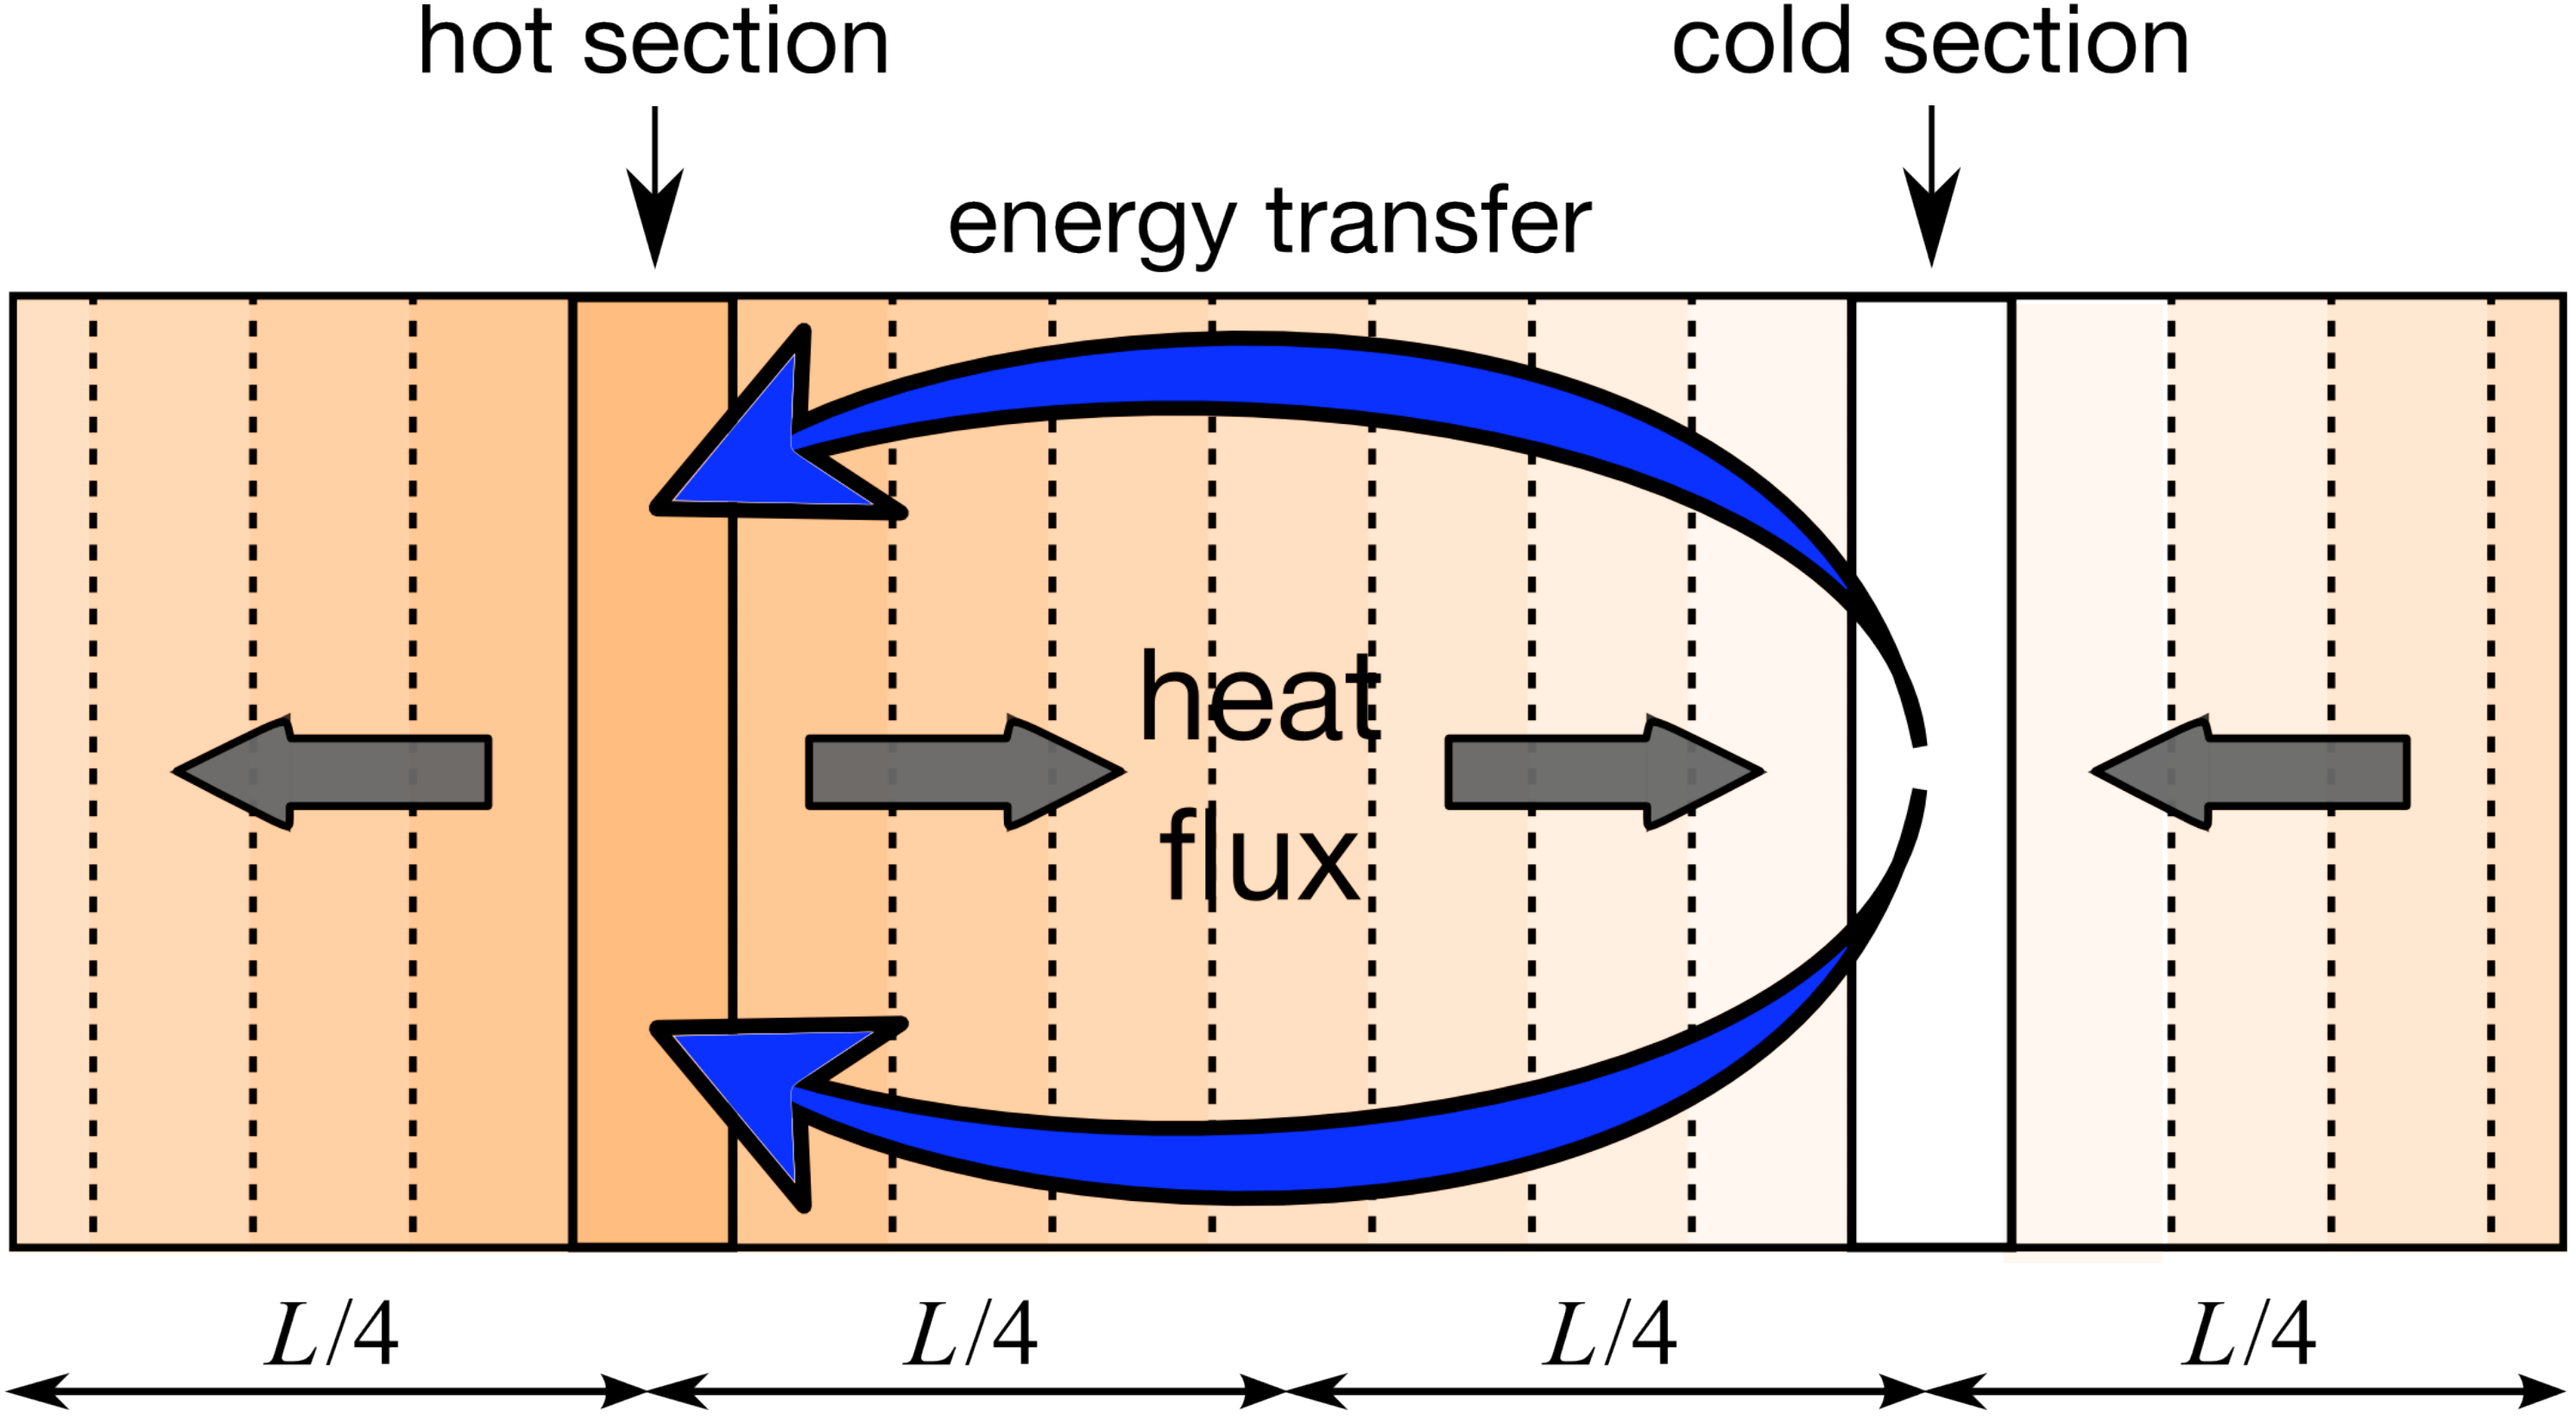
\includegraphics[width=\linewidth]{images/ss_direct_mod.png}
%  \caption{Movement and distribution of heat in the direct method. Orange to white scale represents temperature. Source: \citet{Stackhouse2015}.}
%  \label{fig:ss_direct}
%\end{figure}

From kinetic theory ((REFERENCE??)), conductivities computed by the direct method ($k_L$) are dependent on length of simulation cell,
\begin{equation}
k_{L} = \frac{1}{3} C_{V} v l_{L} \label{length-dep},
\end{equation}

where $C_v$ is the volumetric heat capacity, $v$ is the average phonon drift velocity, and $l_L$ is the phonon mean free path. The finite size of the simulation cell truncates the mean free path, underestimating conductivity compared to that of the bulk material ($k_\infty$). Using results from simulations of varying cell length ($L$), conductivity is extrapolated to a length-independent value (where $b$ is a material dependent parameter),

\begin{equation}
{k_{L}}^{-1} = b L^{-1} + {k_{\infty}}^{-1} \label{linear-extrap}.
\end{equation}

Inverse conductivities from direct method simulations are plotted against corresponding inverse cell lengths. A straight line is fit to the data and extrapolated to the y-axis (at which the inverse cell length equals zero and real length equals infinity), where the intercept gives the inverse of the bulk material conductivity (\citet{Schelling2002}).

%\begin{figure}[h]
%  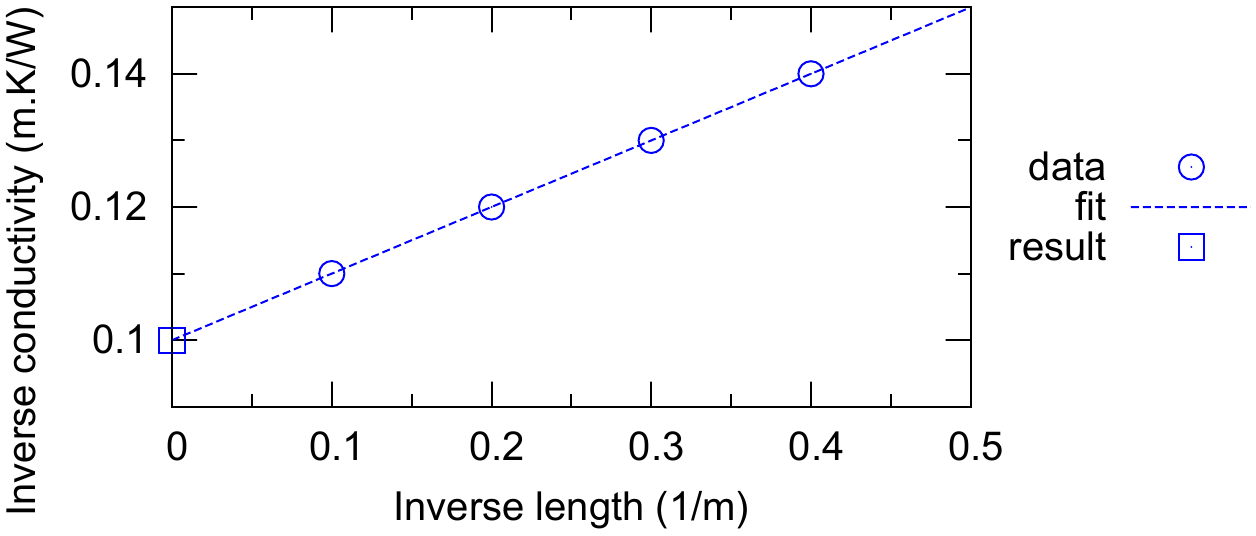
\includegraphics[width=\linewidth]{images/ideal_extrap.png}
%  \caption{Idealised example of linear extrapolation procedure. Inverse computed conductivities are plotted against inverse simulation lengths. Extrapolation to y-axis gives conductivity of an infinite system length, i.e. the bulk material.}
%  \label{fig:ideal}
%\end{figure}

%Computational techniques are not limited by the reproduction of physical conditions like experiments, however they are affected by the size and shape of the simulation cell. The effects of the finite system size available for computation must be checked, as systems with too few atoms are sometimes unable to reproduce the behaviour of the bulk material. If the wavelength of a phonon is too long to fit into a cell, it is not able to transport heat like it should. In the case of the direct method, the length to cross sectional area (CSA) aspect ratio can also matter.

Problems arise when the data do not support a linear trend. There are two effects of finite system size that can cause an individual direct method simulation to diverge away from an inferred/expected linear trend, both of which result in overestimation of the length-dependent conductivity data point. First, when the distance between hot and cold sections (controlled by cell length) is shorter than the MFP, phonons travel ballistically (i.e. without any scattering events) from heat source to sink (\citet{Sellan2010}). Conductivites in shorter length cells are overestimated when this occurs, reducing the gradient of the linear fit and thus underestimating the extrapolated conductivity [[[I NEED TO HAVE SHOWN A FIGURE BY THIS POINT TO MAKE SENSE]]].

For a given length, conductivity is dependent on the CSA, or aspect ratio of the simulation cell. Conductivity is overestimated due to an underestimation of phonon-phonon scattering, from sparse phonon phase sampling in the cross-section compared to the length. Phonons that aren't resolved cannot contribute to phonon-phonon scattering effects. Reduced scattering means heat transport is artificially more efficient than expected from the bulk material. 

THIS CHUNK OF TEXT TOO SPECIFIC TO MY WORK? TOO RESULTSY? MOVE TO RESULTS AND BE MORE GENERAL HERE?

However, the required CSA to abate this FSE is length-dependent. When the CSA is smaller than required for all cell lengths (e.g. 1x1 [FIGURE]), all conductivities are overestimated (\citet{Thomas2010}? NANOTUBE DIAMETER RATHER THAN CSA). As the CSA is increased (e.g. to 2x1 and 2x2), a systematic shift for all data points (and thus the extrapolated result) to lower conductivities (higher inverse conductivities) is observed. It is at this point that the short cells, with their lengths of similar order (i.e. 6-16 unit cells), will report conductivities converged with respect to CSA. Assuming these cells are sufficiently long to avoid the ballistic phonon transport (BPT), a linear fit can be extrapolated to obtain conductivity (the case at 4000~K). 

The convergence is not necessarily observed for the longer cells however, where they might show overestimated conductivities compared to the fit through the short cells (\cite{Hu2011}). This would cause a fit through all data points to be steeper than it should, again increasing the extrapolated result.  [[[HOPEFULLY THIS IS TRUE]]] I can show that increasing CSA does not change the computed conductivity at short lengths, but does reduce values from longer cells and bring them into alignment with the expected fit.

The effect of FSE on conductivity results depends on the magnitude of conductivity/phonon MFP/physical conditions. At low kappa/low MFP/high T/ (my 4000~K), no BPT is observed, and short cells (>16 unit cells) can be used for extrapolation. In fact, short cells must be used to extrapolate, unless CSA considersations are made to ensure convergence of long cell results.

At high kappa/high MFP/low T (my 1000~K), BPT must considered at the shorter cells (just 6?). Effectively there is a "sweet-spot", a window of cell lengths for a given CSA that produce consistently-converged results. Long cells outside of the window require a larger CSA, short cells outside show BPT. At 4000~K the lower limit of the window is smaller than the minimum cell length considered, and the upper limit is between 16-24 unit cells. For 1000~K the lower limit of the window moves inside the simulated cell length range around 6-8 unit cells (OR MORE?). The upper limit of the window appears to be larger than 96 unit cells, including all long cells up to this value produces an extrapolation in agreement with GK.


%%%MOVE TO 3

(MOVE TO METHOD?) By comparing results with the Green-Kubo method, we will constrain the cell lengths in the linear extrapolation region to mitigate these effects. 

(MOVE TO RESULTS?)We have investigated this effect by varying CSA for a range of cell lengths, extrapolated conductivity decreases and eventually converges with CSA. We will use the smallest area that produces the converged conductivity for computational efficiency. 









\subsection{\label{sec:theory.gk}Green-Kubo method (remove this subsection header later)}

RETHINK FIGURES - WHICH DATA TO USE

TALK ABOUT GK FSE - WHAT AND WHY

The Green-Kubo method uses auto-correlation functions (ACFs) to quantify time-dependence of heat fluxes (shown in Figure~\ref{fig:gk_acf}, and Equation \ref{acf-j}), in a simulation cell of roughly cubic dimensions (WHY??) and spatially-consistent average temperature. Instantaneous heat fluxes can be used to determine how energy is dissipated within a system, where brief flux events mean heat is transferred quickly indicating high thermal conductivity (and vice versa, BUT IS THIS TRUE???). Auto-correlation is performed over the net heat flux series in each crystallographic direction, for a timescale up to a chosen correlation length.

\begin{equation}
ACF_i = \left \langle J_i(0) \cdot  J_i(t) \right \rangle,
\label{acf-j}
\end{equation}
%%%%%%%%%%%%%%%%
\begin{figure}[h]
  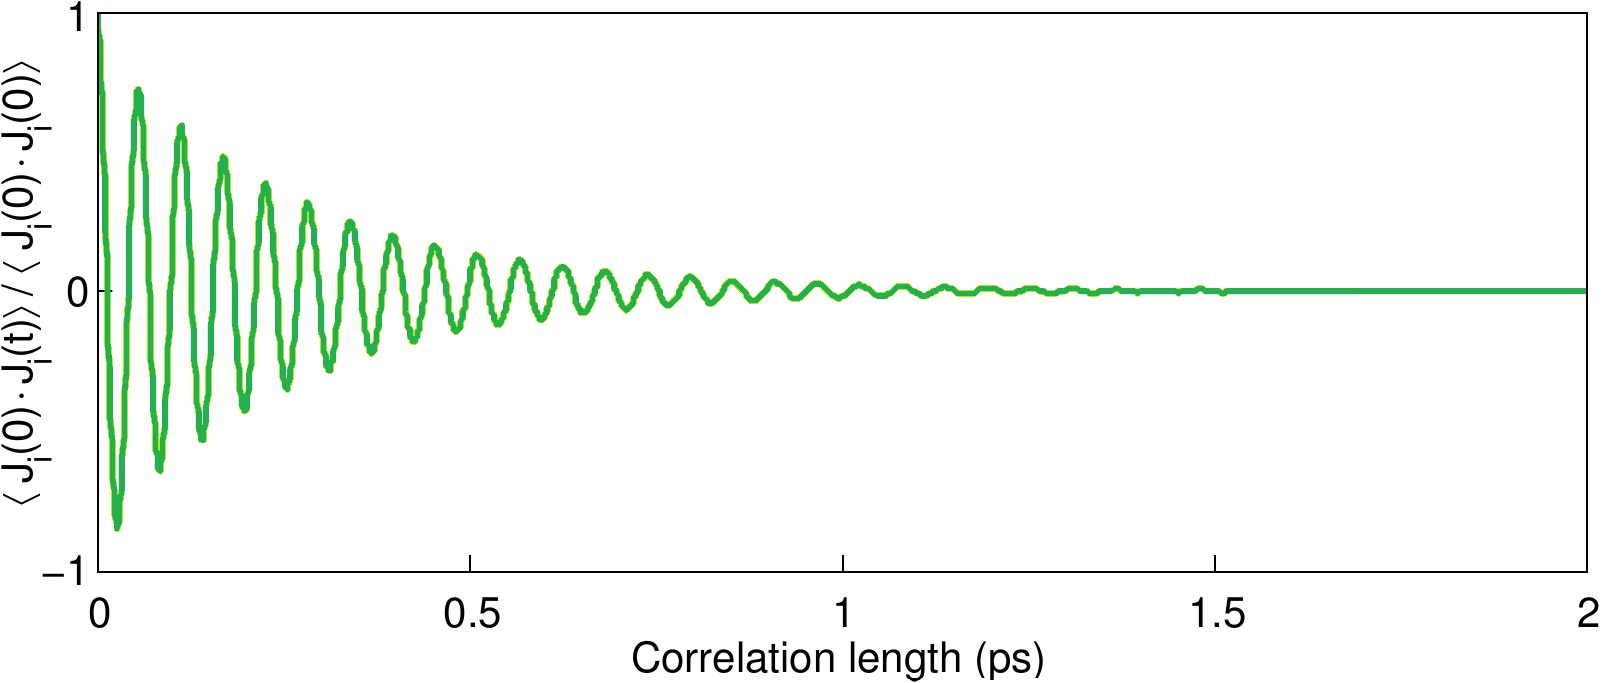
\includegraphics[width=\linewidth]{images/gk_acf.png}
  \caption{Normalised ACF. Correlation is taken over a longer length than shown on this plot (10 ps, see Figure 8 below), however the function decays to less than 1\% of its initial value at 2~ps. It continues to oscillate about zero, with a positive average value.}
  \label{fig:gk_acf}
\end{figure}
%%%%%%%%%%%%%%%%
where $i$ specifies direction, $J$ is heat flux, and $t$ is the correlation length. The integral of heat flux ACF is proportional to thermal conductivity via the Green-Kubo equation (see Figure~\ref{fig:gk_int} and Equation \ref{gk-int}), 

\begin{equation}
\kappa_i = \frac{V}{k_{B}T^2} \int_{0}^{\infty} \left \langle J_i(0) \cdot  J_i(t) \right \rangle dt ,
\label{gk-int}
\end{equation}
%%%%%%%%%%%%%%%%
\begin{figure}[h]
  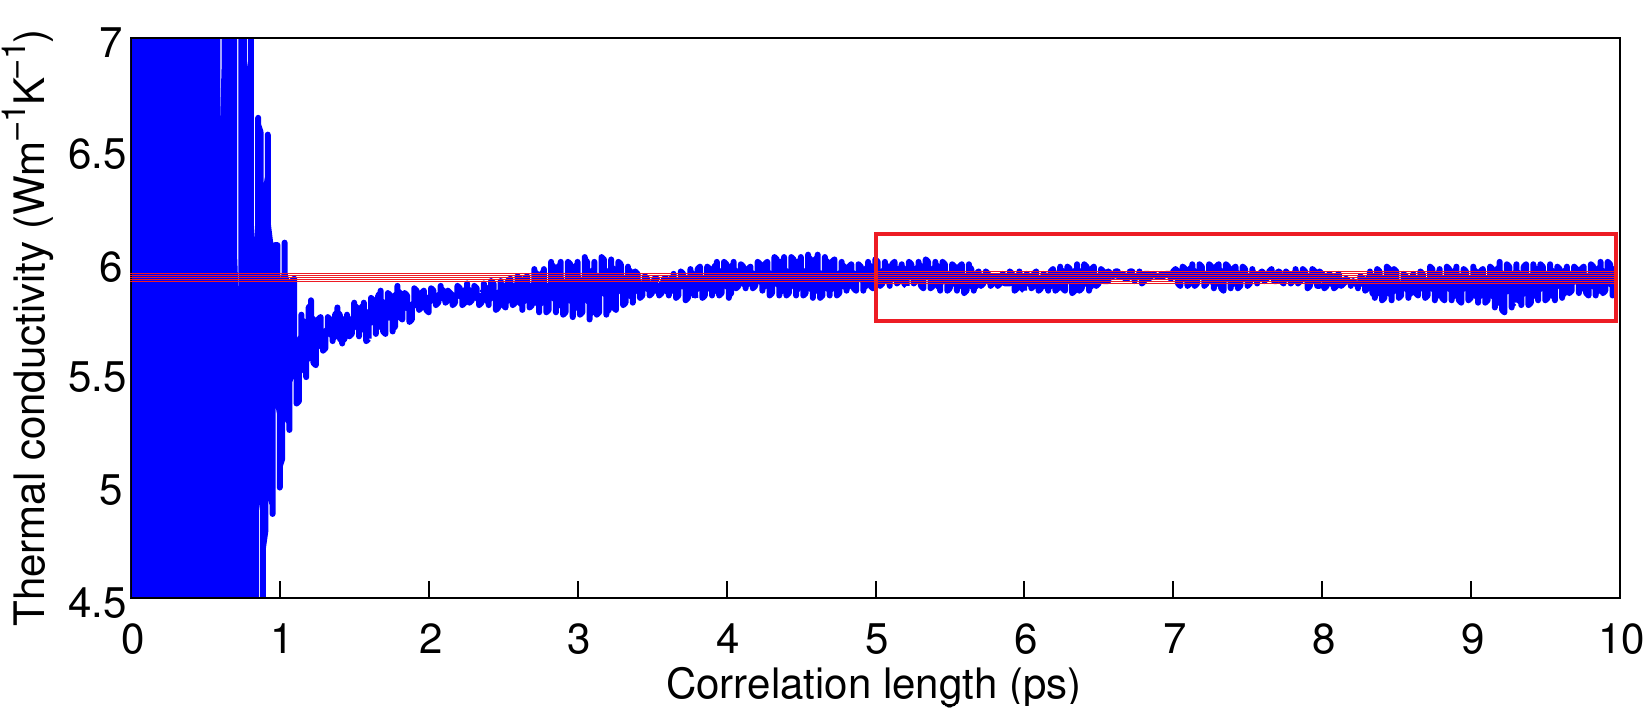
\includegraphics[width=\linewidth]{images/gk_int.png}
  \caption{Integrated ACF, multiplied by constants to get thermal conductivity. Large variation in the first 1 ps corresponds to the correlation time where the ACF is unconverged (still decaying / large oscillations). Thermal conductivity is averaged from correlation time of 5~ps - 10~ps (region in red box).}
  \label{fig:gk_int}
\end{figure}
%%%%%%%%%%%%%%%%
where $V$ is the simulation cell volume, $k_B$ is the Boltzmann constant, and $T$ is the average temperature of the system. In this study we use Green-Kubo results as an independent check on the direct method, as they do not have the same finite size-effects. Obtaining a converged conductivity result simply depends on using a large enough cell volume / number of atoms. 

The individual integrals obtained from the Green-Kubo show variation from the average combined integral on the order of the mean. Many simulations from different intital temperature conditions are required in order to ensure good sampling of conductivity, as well as ensuring the computation time for each is long enough for convergence. This makes Green-Kubo a computationally expensive method, especially for large systems.

The ACF should decay to zero as correlation time tends to infinity, however noise in the ACF prevents this. This will ultimately cause the integral to diverge/drift on long timescales. \citet{Howell2012} fits a series of exponential decays to their ACF, forcing the expected decay to zero and subsequent (constant) integral convergence. This is represents a significant improvement on the conductivity estimate at long correlation lengths, but is mostly similar with the un-fit integrals early in the correlation. (INTEGRAL DRIFT FIGURE, JUST THE ONE INTEGRAL FOR 100PS)

(STACKHOUSE 2010 REFERENCES Volz and Chen 2000; Sun and Murthy 2006)





\section{\label{sec:methodology}Methodology}

ENOUGH INFO FOR REPRODUCIBILITY !!!

WHAT I HAVE DONE / FOR REPRODUCIBILITY. SETUP STUFF, BUT CONDUCTIVITY / FINITE SIZE EFFECT RESULTS GO IN RESULTS SECTION


Using the classical molecular dynamics code LAMMPS(\citet{Plimpton1995}) (Large-scale Atomic/Molecular Massively Parallel Simulator), we calculate lattice thermal conductivities and constrain effects of finite simulation size. With the interatomic potential of \citet{Oganov2000} we simulate bridgmanite (MgSiO$_3$ perovskite), the predominant phase in the lower mantle ($\sim$75\%). 

To assess the finite-size effects within bridgmanite, we use larger simulation cells than those employed in previous studies (BRIDG STUDIES OR FSE STUDIES?). The atom counts associated with these cells (the largest cell considered having over 100,000 atoms) means an ab initio study would be impractical, necessitating the use of interatomic potentials. We expect the potentials to represent the finite size effects well, even if computed conductivities may inaccurate compared to first-principles calculations.

WHY OGANOV? 

WHAT CUTOFFS?

We present our approach for the direct and Green-Kubo methods, and show our calculations are converged with respect to simulation time (also temperature gradient and correlation length respectively - AWKWARD BRACKETS) [[[  DO SIMULATION TIME CONVERGENCE FOR GK TOO ]]]. The finite-size effect analysis for both methods can be found in Section.~\ref{sec:results}, along with a results comparison.

NPT-NVT-NVE PROCESS, BOTH METHODS

BAROSTAT-THERMOSTAT-SIMULATION

[[ THIS PARAGRAPH IS DUMB, I DON'T THINK IT NEEDS TO BE IN PAPER ]] We ensure all calculations are run for a sufficient length of time for the conductivity value to converge. When conductivity fails to converge it means either the simulations needs to be run for longer (unlikely with our nanosecond-scale classical calculations), or the system temperature has drifted. When NVE simulations are run for a long time there is noticable drift in the average system temperature (due to numerical approximations in the equation of motion), which in turn causes drift in the computed conductivity. 




\subsection{\label{sec:method.direct}Direct method}

The simulation supercell is split into sections along its length, each half a unit cell wide. Two of these sections, half the supercell length apart, are designated as the heat source and heat sink. We measure (HOW?) the temperature in all sections to obtain the temperature gradient. Heat flows in both directions from the hot section because of cell periodicity [NEED DIRECT METHOD DIAGRAM BY THIS PARA], meaning there are two temperature gradients to average. Where L is supercell length in unit cells and S (= 2L) gives the number of sections, we obtain S/2 + 1 temperature points to fit the gradient. Because the temperature gradient is non-linear around the heat source and sink, we ignore S/12 sections (rounded to nearest integer) from both ends of the temperature gradient. For a given simulation cell we fit S/3 + 1 points to obtain the temperature gradient. We use a minimum supercell length of 6 unit cells (12 sections, 5 data points), in order for sufficient fitting of the temperature gradient. [HOW NECESSARY IS THIS PARA, VERY JARGONY]

(MOVE TO RESULTS?) Changing the width of the heated sections has no effect on the conductivity result. Furthermore, changing the width (and thus number) of temperature bins has no effect on the sampled gradient, assuming resolution is large enough to capture the non-linear region around the heat source/sink.

An important factor for utilising the direct method is maintaining a sensible temperature gradient where Fourier's law remains valid, i.e. conductivity is constant along the length of the cell. Thermal conductivity is strongly temperature-dependent at upper lower-mantle conditions (1000~K), it is therefore undesirable to have substanially different conductivities as a of function of temperature across the cell. The opposite case is also true, the difference in temperature between hot and cold sections must be larger than the uncertainty in the average system temperature. 

We typically observe fluctuations in temperature of around $\pm$50~K during temperature equilibration, and look for temperature increases/decreases on the order of 10\% the mean temperature. We control the magnitude of the gradient by altering the interval at which heat is exchanged. To produce the desired gradients we find shorter intervals are required as cell length decreases, cross-sectional area increases, and system equilibrium temperature decreases. 

%Figure \ref{fig:swap_int} (larger y-axis range?) shows conductivity as a function of swap interval for a 6x2x2 system at 136~GPa and 1000~K. Values are erratic for high interval / low temperature range swaps (right), and converge with decreasing swap interval (left). An interval around 10~timesteps produces suitable results for these system conditions, whilst exhibiting a sensible temperature range for the reasons mentioned above. 
% the finite-distance approximation associated with molecular dynamics

%This process is accelerated when heat is exchanged often, an important thing to check for when processing data.

%\begin{figure}[h!]
%  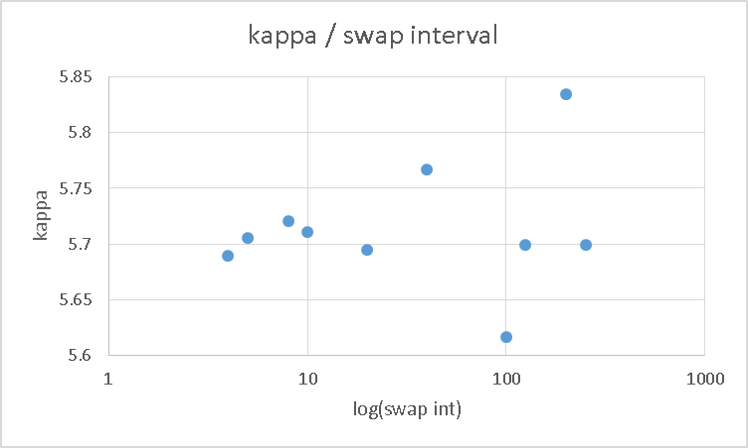
\includegraphics[width=\linewidth]{images/swap_int.png}
%  \caption{ADD IN TEMPERATURE INFORMATION}
%  \label{fig:swap_int}
%\end{figure}

% NOT NEEDED
%\begin{figure}[h!]
%  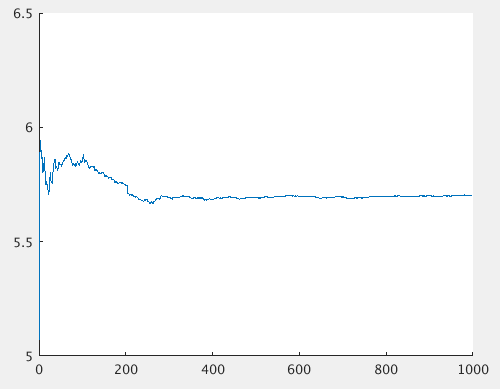
\includegraphics[width=\linewidth]{images/kappa_conv.png}
%  \caption{conductivity versus simulation time direct method. converged after 300ps. DO I NEED THIS FIGURE?}
%  \label{fig:kappa_conv}
%\end{figure}


















\subsection{\label{sec:method.gk}Green-Kubo method}

The bridgmanite unit cell does not have cell dimensions resembling a cube (a:b:c = 1:1:1.4), so we use supercell structures of 3x3x2, 4x4x3, 5x5x4, 6x6x4 etc. to make an approximately cubic simulation cell. Temperature initialisation (NVT) of 1~ns is run to ensure convergence of system pressure and temperature. To obtain heat flux auto-correlation functions, a simulation for each initial temperature condition is run for X~ns, with 9 successive repeats for a total of 10 jobs. This gives 10 ACFs from each initial condition. Simulation runs are split in this manner to be feasible computationally, and also to provide enough samples for ensemble averaging statistics (???).

3x3x2 - X = 10~ns, for 20 inital conditions - 2~$\mu$s total time

4x4x3 - X = 10~ns, for 30 inital conditions - 3~$\mu$s total time

5x5x4 - X = 5~ns, for 20 inital conditions - 1~$\mu$s, X = 1~ns, for 70 inital conditions - 0.7~$\mu$s, 1.7~$\mu$s total time

6x6x4 - X = 1~ns, for 80 inital conditions - 0.8~$\mu$s total time

THIS INFO IN A TABLE, OR JUST GIVE FOR THE RELEVANT VOLUME?

I DON'T LIKE THE INCLUSION OF ALL THE ABOVE INFORMATION

In this study we compute ACFs up to correlation lengths of 100~ps, with (100,000) 1~fs timesteps. This length is longer than required but selected as a proof of concept to show convergence in the conductivity result, additionally to display the extent and behaviour of drift in the integrals for long correlation times. We show in Figure \ref{fig:acf_decay} that the magnitude of the ACF decays to much less than 1\% of its initial value around a correlation time of 1~ps, inferring the start of convergence for the integral and thus conductivity. (ACF FIGURE FOR CORREL < 10PS?, RUNNING AVERAGE SHOWS CONVERGENCE) 

%ORIG - ACFs produced by each simulation are integrated seperately, after which the integrals are averaged into a single series with uncertainty (standard deviation of the mean, \ref{fig:664z_100ps}). This process is performed for heat fluxes in each crystallographic direction, allowing analysis of anisotropy and finite system size effects. We obtain a conductivity value from the combined integral by averaging a window between correlation times of 2-10~ps (for 136~GPa, 4000~K [THIS WILL NEED TO BE CHANGED]). Windows are chosen to capture a flat, converged region of the integral, or the section just after the 'bottleneck' if convergence is not obvious (\ref{fig:664z_10ps}, but show window, and example of bottleneck?). We find correlation time of 2-10~ps to be long enough for good sampling of the integral, and short enough to ignore the aforementioned drift-effects. (INTEGRAL FIGURE WITH UNCERTAINTY FOR <10PS?, POINT TO CONVERGENCE, SHOW SMALL ZOOM OUT OF SAME GRAPH UP TO 100PS. SOME WAY TO COMBINE WITH ABOVE FIGURE)

ACFs produced by each simulation are integrated seperately, and averaged into a single series. This process is performed for heat fluxes in each crystallographic direction, to allow analysis of anisotropy and finite system size effects.  From this combined integral we pick a window of correlation lengths to capture a flat, converged region (or the section just after the 'bottleneck' if convergence is not obvious). This correlation length window is then applied to all N integrals constituent to the combined series, giving N integral averages and corresponding standard deviations. A weighted average is then taken of these data points, to give a single value with uncertainty. This value is directly proportional to thermal conductivity, as given by EQUATION XXX.

Considering bridgemanite at lower mantle conditions, we find correlation time windows in the range of 2-30~ps to be suitable. At the low-end, this allows the initial high-variability in integral value to be ignored. At the high-end, the time is long enough for good sampling of the integral, but short enough to ignore the drift-effects. The magnitude and range of the window typically increases with conductivity (or with decreasing temperature etc.), e.g. 2-10~ps at 4000~K, and 10-30~ps at 1000~K.



%(SELLAN2010) Average over time and multiple simulations of different initial conditions. The total simulation time should be many times larger than the largest phonon relaxation times that dominate thermal conductivity, in order to accurately predict a converged value of the integral.

AAARRGH!!! - CONVERGENCE OF KAPPA WITH SIMULATION TIME - AAARRGH!!! 

DONT NEED ALL THESE GRAPHS

\begin{figure}[h!]
  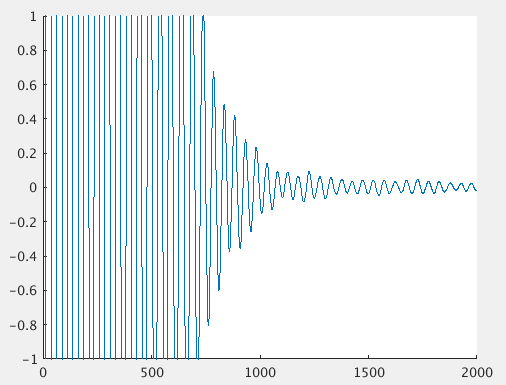
\includegraphics[width=\linewidth]{images/acf_decay_percent_correl.png}
  \caption{normalised acf in percent against 2ps correl. 1 on y-axis = 1\%}
  \label{fig:acf_decay}
\end{figure}

\begin{figure}[h!]
  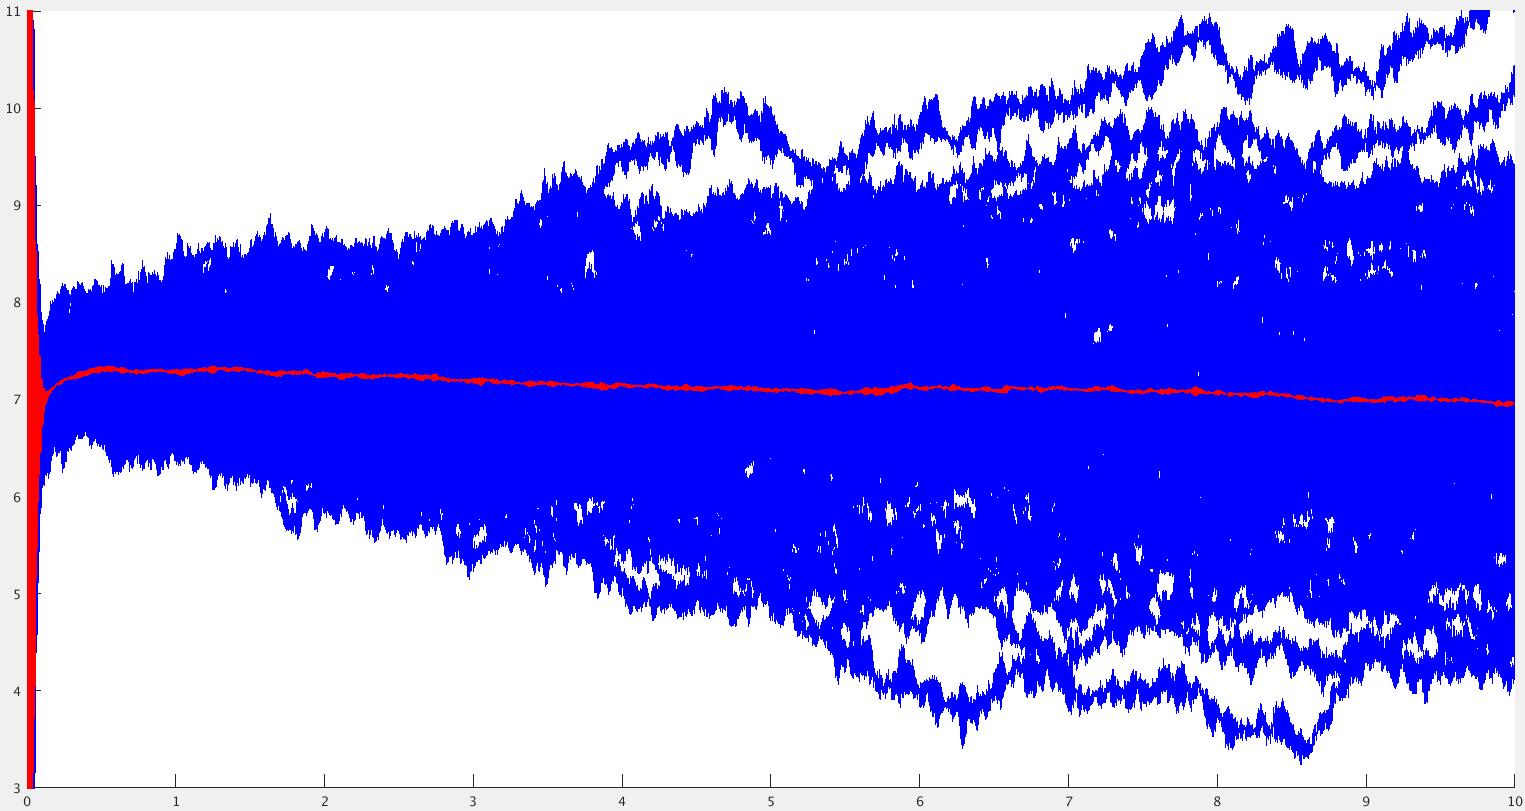
\includegraphics[width=\linewidth]{images/4x4x3_01-z-ints.png}
  \caption{kappa against 100ps correl}
  \label{fig:int_drift}
\end{figure}

\begin{figure}[h!]
  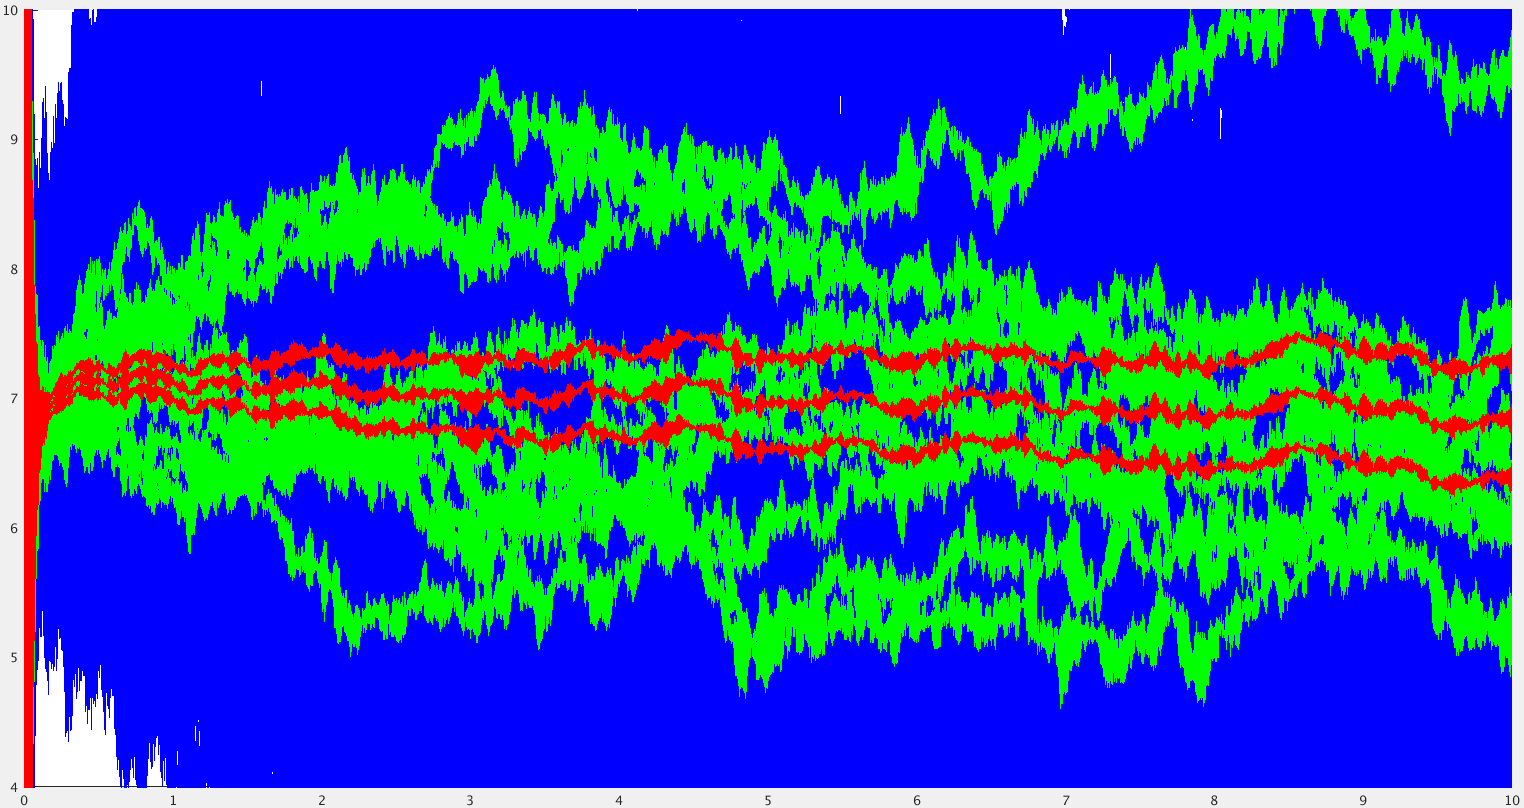
\includegraphics[width=\linewidth]{images/6x6x4_01-z-stddev.png}
  \caption{kappa w/ uncertainty against 100ps correl. green series is all runs from each initial condition combined}
  \label{fig:664z_100ps}
\end{figure}

\begin{figure}[h!]
  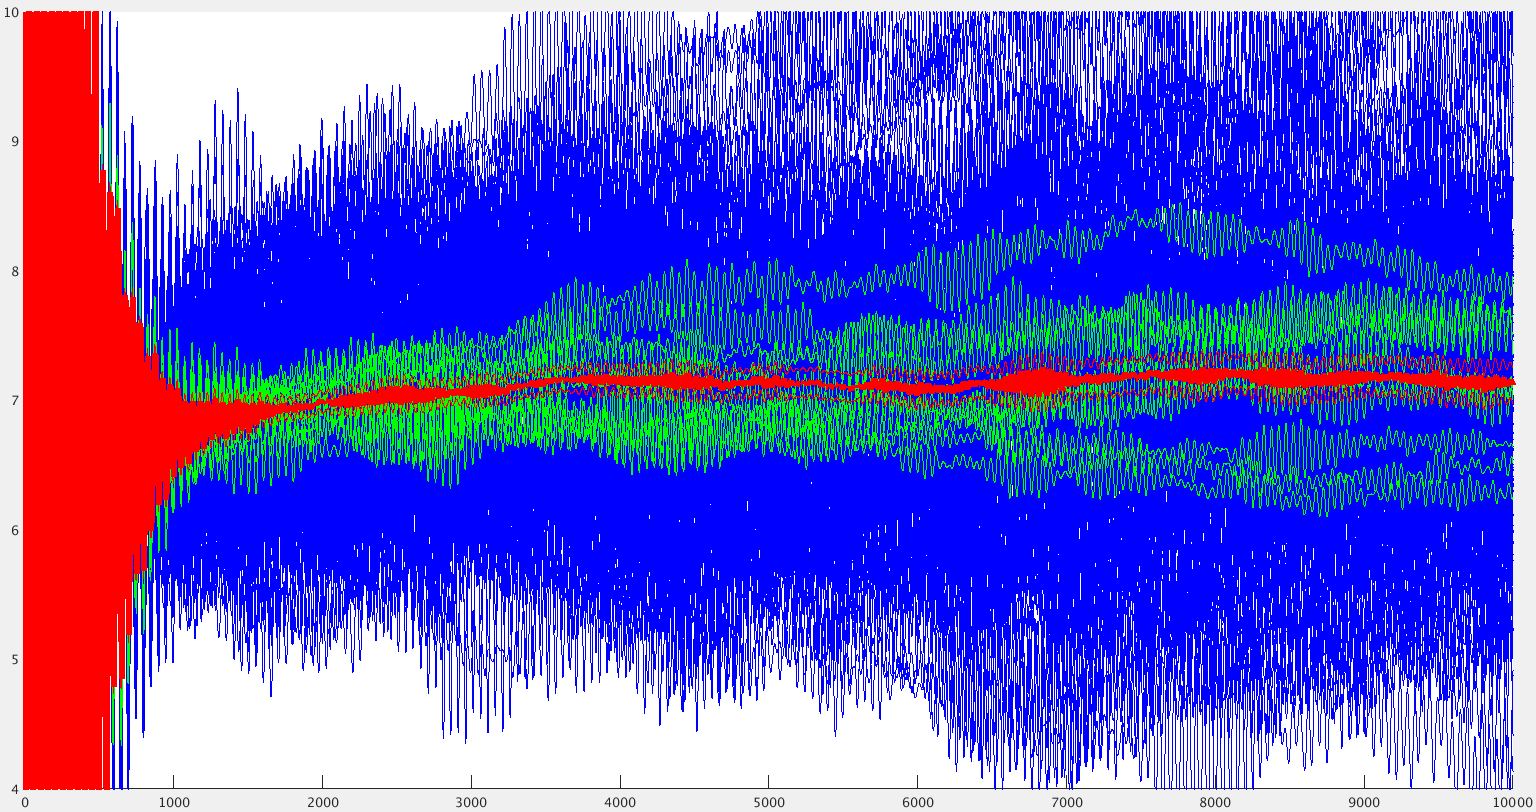
\includegraphics[width=\linewidth]{images/6x6x4_01-z-stddev_2-10ps.png}
  \caption{kappa w/ uncertainty against 10ps correl. shorter time scale than previous figure. flat region from 4-10ps. DON'T NEED ALL THESE GK FIGURES}
  \label{fig:664z_10ps}
\end{figure}
















\section{\label{sec:results}Results}

LOTS OF QUANTIFYING

\subsection{\label{sec:results.gk}Green-Kubo method}

A supercell volume of 3x3x2 (((REFER TO GRAPH, WILL NEED 1000K TOO))) fails to reproduce conductivities on the same order as the larger cells for all directions. We identify 4x4x3 and larger cells as being converged with respect to cell volume (((PROBLEMATIC STATEMENT, NOT CONVINCING, BY WHAT METRIC?))). This a useful result in terms of computation efficiency, as 6x6x4 supercells are 3 times as large (VOLUMOUS? REFERENCE ATOM COUNT?) as 4x4x3.

\begin{figure}[h!]
  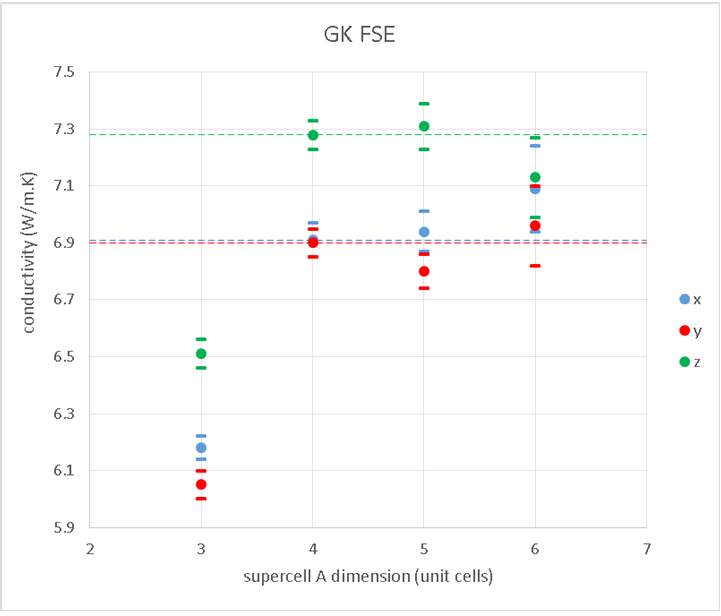
\includegraphics[width=\linewidth]{images/gk_fse_draft.png}
  \caption{kappa vs. volume, all directions. dashed lines show values at 4x4x3, the chosen volume, for comparison. change x-axis to atom count, or number of constituent cell?}
  \label{fig:gk_fse}
\end{figure}








\subsection{\label{sec:results.direct}Direct method}

MFP DEPENDENT FSE, PROVE DIFFERENCE. 

When determining finite-size effects, it is important to consider the scenario with largest phonon mean-free paths. Phonon MFPs are largest at low temperatures (beyond the Debye temperature) and high pressures. In light of this we consider pressure of 136~GPa and temperatures of 1000~K and 4000~K. 136~GPa / 4000~K represents the expected conditions of the core-mantle boundary, whereas 136~GPa / 1000~K is unphysical in the context of the Earth but maximises MFP.  UPDATE - GK RUINS EVERYTHING

By computing conductivities across a range of cell lengths we show that direct method simulations with small cross-sectional areas fail to produce converged results with respect to larger CSAs. Without considering any extrapolation, it is clear that small CSA cells overestimate conductivity (Figures \ref{fig:direct_length_graph_4000} \& \ref{fig:direct_length_graph_1000}) at conditions of both 1000~K and 4000~K. On both figures the results for cells with CSA 2x2 and larger plot close to on top of each other. Producing the same results as 8x8 cells, we conclude that cells with CSA of 2x2 are suitable for direct method simulations of bridgmanite.

\begin{figure}[h]
  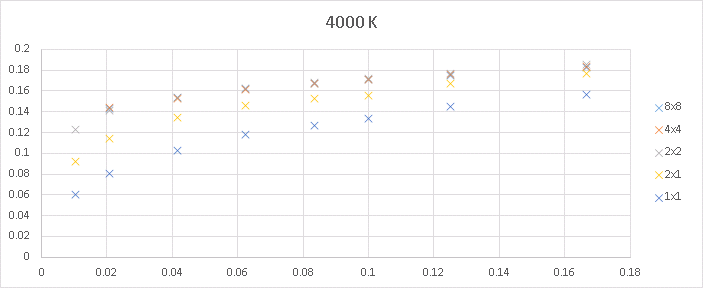
\includegraphics[width=\linewidth]{images/direct_length_graph_4000.png}
  \caption{inverse conductivity against inverse length at 4000K. each series is a different CSA}
  \label{fig:direct_length_graph_4000}
\end{figure}

\begin{figure}[h]
  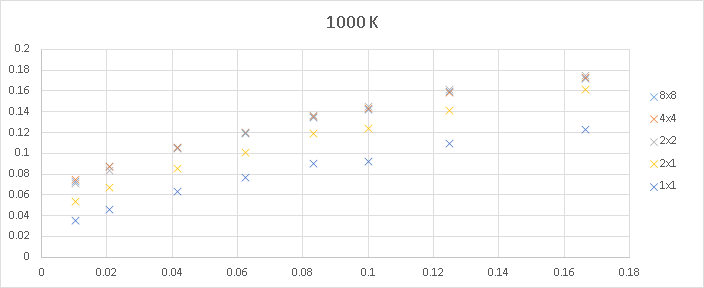
\includegraphics[width=\linewidth]{images/direct_length_graph_1000.png}
  \caption{inverse conductivity against inverse length at 1000K. each series is a different CSA. COULD TRY AND COMBINE THESE FIGURES, SIMILAR Y-AXIS, MIGHT BE MESSY}
  \label{fig:direct_length_graph_1000}
\end{figure}

Now considering CSAs of 2x2, we examine the divergence of conductivity result with cell length from an expected linear trend (Figure \ref{fig:direct_length_graph}). As mentioned in Section \ref{sec:theory.direct}, cells that are too long or short cause a conductivity result to be overestimated. At 4000~K we find that cells up to 24 unit cells length ($<$0.06 in inverse length) produce a reasonably linear trend. At this condition, there is no reasonable overestimation due to short cells and ballistic phonon transport. However at 1000~K where the MFP is longer, a cell of length 6 unit cells (inverse length 0.167) produces conductivity larger than expected. The same long-cell divergence is found $>$24 unit cells length, the onset of insufficient phonon sampling. For all direct method simulations of bridgmanite at lower mantle conditions, we recommend employing cell lengths of 8~-~$<$24 unit cells. Due to the increasing computational cost associated with cell length (especially for ab initio methods), we recommend the longest cells be 16 unit cells. FINITE SIZE EFFECTS INCREASE WITH MFP/KAPPA

\begin{figure}[h]
  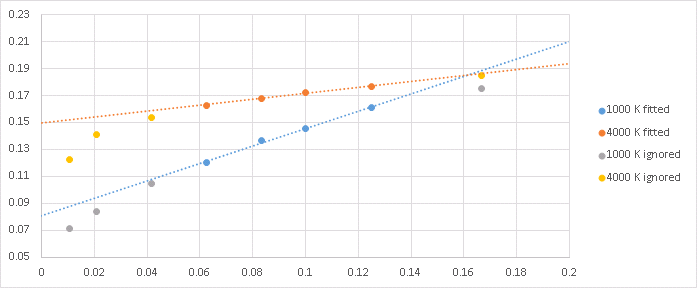
\includegraphics[width=\linewidth]{images/direct_length_graph.png}
  \caption{off-colour data points are not fit. Although the 1000~K data points look closer to the linear trend, they are further in magnitude due to the nature of the inverse y-axis.}
  \label{fig:direct_length_graph}
\end{figure}

\begin{figure}[h]
  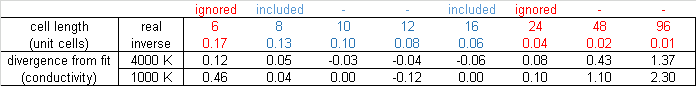
\includegraphics[width=\linewidth]{images/direct_length_table.png}
  \caption{MAKE THIS INTO A LATEX TABLE OBVIOUSLY}
  \label{fig:direct_length_table}
\end{figure}

Now we consider CSA of 2x2 and supercell lengths of 8, 10, 12, and 16 unit cells for comparison with the results from Green-Kubo. After performing a weight least squares regression (extrapolation) on the direct method results, we obtain a conductivity with uncertainty. Figure \ref{fig:gk-direct} shows the extrapolation and Green-Kubo result (at x~=~0). They agree within error, meaning we have chosen a suitable set of criteria for working with direct method results. DO I NEED TO PROVE THAT OTHER LENGTHS/EXTRAPOLATIONS DON'T MATCH GK? FINE AT HIGH T / SHORT MFP, LOW T / HIGH MFP NEEDS LONGER CELLS TO EXTRAPOLATE, OR MORE SHORTER CELLS IGNORED.

\begin{figure}[h!]
  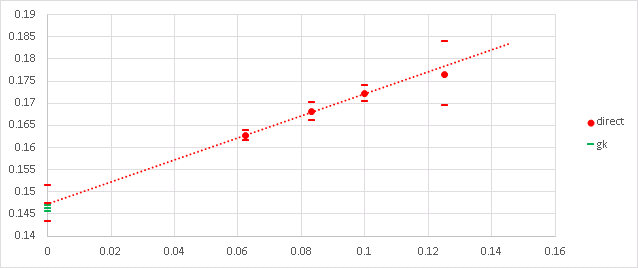
\includegraphics[width=\linewidth]{images/gk-direct-2.png}
  \caption{The results of Figure 9 for cross-section of 2x2 and lengths ≤ 16 unit cells. Diagrams of cell geometry are shown, with dimensions in unit cells and the number of atoms. Green-Kubo result is plotted on the y-axis for comparison with extrapolated direct method conductivity. WEIGHTED FIT DOESN'T LOOK LINEAR, INCREASE Y-AXIS RANGE?}
  \label{fig:gk-direct}
\end{figure}



%As it is inappropriate to fit non-linear data, we ignore conductivity results from the long cells and perform the extrapolation only where a linear trend is suitable.

%\begin{figure}[h]
%  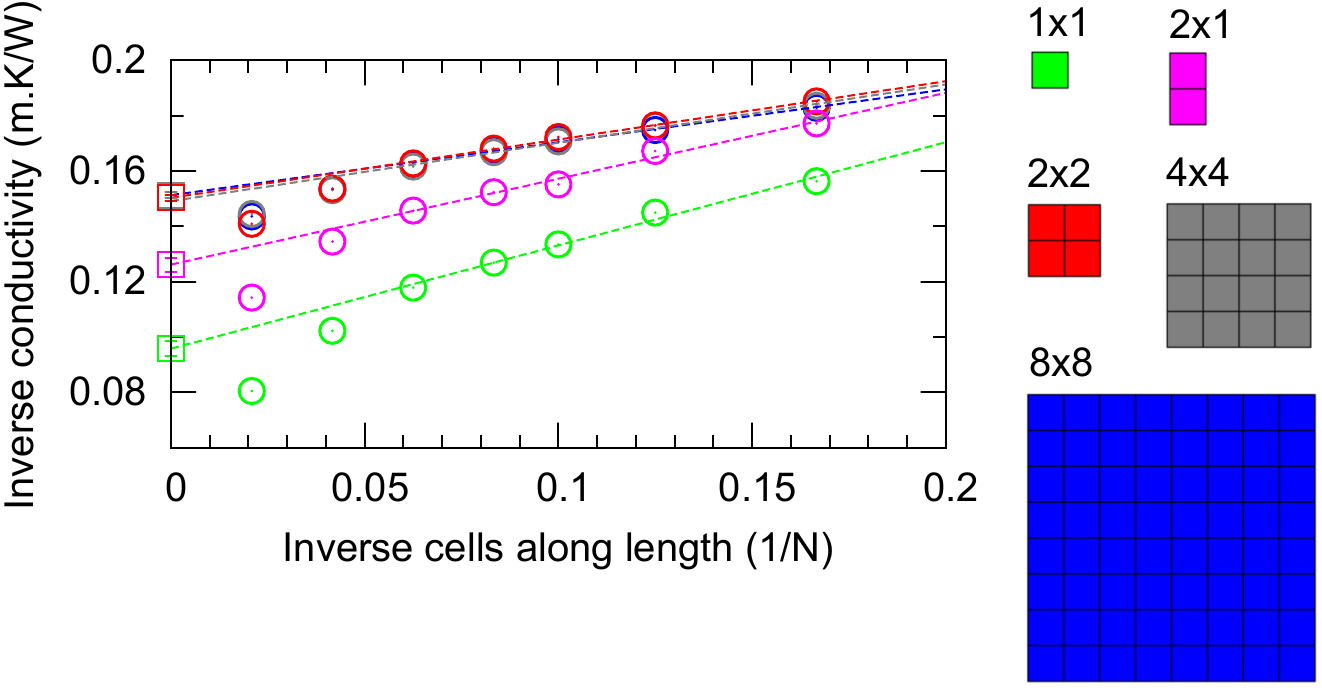
\includegraphics[width=\linewidth]{images/all_data.png}
%  \caption{Compilation of direct method thermal conductivities across a range of cell shapes at 4000 K and static pressure of 136 GPa. Different cross-sections are displayed by the colour of the series, diagrams of which are shown in the legend (right). From right to left, data points correspond to lengths of 6, 8, 10, 12, 16, 24, and 48 unit cells. Inverted axes facilitate the extrapolation of conductivity to bulk material.}
%  \label{fig:all_data}
%\end{figure}


SCALING LAW / THEORETICAL MODEL

PROBABLY SHOULD MENTION THE VALUE OF THE RESULT?

PREVIOUS WORK :(







\section{\label{sec:summary}Summary and conclusion}

For bridgmanite (at conditions representing the lower mantle), we show that use of the direct method for calculation of thermal conductivity will lead to an overestimate if the simulation cell is too long (\textgreater 16 unit cells, 4000 ONLY!!!). Small cross-sectional areas (\textless 2x2 unit cells) also overestimate the thermal conductivity. This informs future work using Density Functional Theory, and will allow a model of lower mantle conductivity considering composition to be established [[[OOPS]]].

(ASSUMING THE RESULTS ARE CORRECT AND AGREE WITH GK) We see the non-linear region as described by \citet{Sellan2010} for the cell length of 6 unit cells at 1000~K, which has individually higher conductivity than expected from the linear fit through data points corresponding to lengths of 8-16 unit cells. When included in the extrapolation, this reduces the gradient of the fit, raising the intercept and thus causing conductivity to be underestimated. At temperature of 4000~K, the 6 length cell is inline with the fit through other cells with length less than 16 unit cells. As the ratio of cell length to phonon MFP increases with temperature, we believe the onset of divergence as described by Sellan et al. moves to the right (??? - MENTION ACTUAL EFFECT - QUANTIFY RATHER THAN REFERENCING GRAPH). A shorter MFP needs shorter cell lengths to display divergent conductivity, of which we have not sampled (at high temperature). DOING THE DIRECT METHOD WITH CELLS OF LENGTH LESS THAN 6 UNIT CELLS AT ANY TEMPERATURE IS A BAD IDEA BECAUSE ... 

We find conductivity is definitely dependent on CSA, but we were not able to increase CSA enough to eliminate aspect ratio-dependent divergence as reported by \citet{Hu2011}. This does support our conclusion ignoring long cell lengths however, in order to keep the aspect ratio within a reasonable limit and ensure a linear fit is extrapolated. (EVEN THOUGH 48x8x8 HAS A SMALLER RATIO than 8x2x2?)

(WAFFLE ALERT) Ignoring the specifics of this study, we stress the importance of performing finite-size analysis when performing direct method calculations.  Direct method cells spanning a range of lengths must be considered to find the linear regime for extrapolation. Cross-sectional area must be increased until the conductivity result converges. The same can be said about the Green--Kubo method, where the result converges with increasing volume. These effects vary with phonon mean-free path, sensitive to pressure, temperature, and compositional variations such as impurities. Completing finite-size effect analysis at conditions with the largest phonon mean-free path / thermal conductivity ensure all other conditions represent converged results. We believe classical molecular dynamics with interatomic potentials to be an excellent way of quantifying these effects quickly, performing ab initio methods (SHOULD I TAKE THIS SENTENCE OUT, NO PROOF OF THIS CLAIM).

FUTURE WORK?

\begin{acknowledgements}
Thank you NERC

"We also acknowledge the use of high performance computing provided by Advanced Research Computing at the University of Leeds."

ANDREW HAS SOMETHING TO ADD (AMW IRF from NERC w/ grant code)

STEPHEN HAS SOMETHING TO ADD (LLSVP Grant from NERC / MSRC / ????)
\end{acknowledgements}

\bibliography{paper1}



\end{document}


